\documentclass[tikz,border=8pt]{standalone}
\usepackage{amsmath,amssymb}
\usetikzlibrary{arrows.meta,automata,positioning,quotes}
\begin{document}
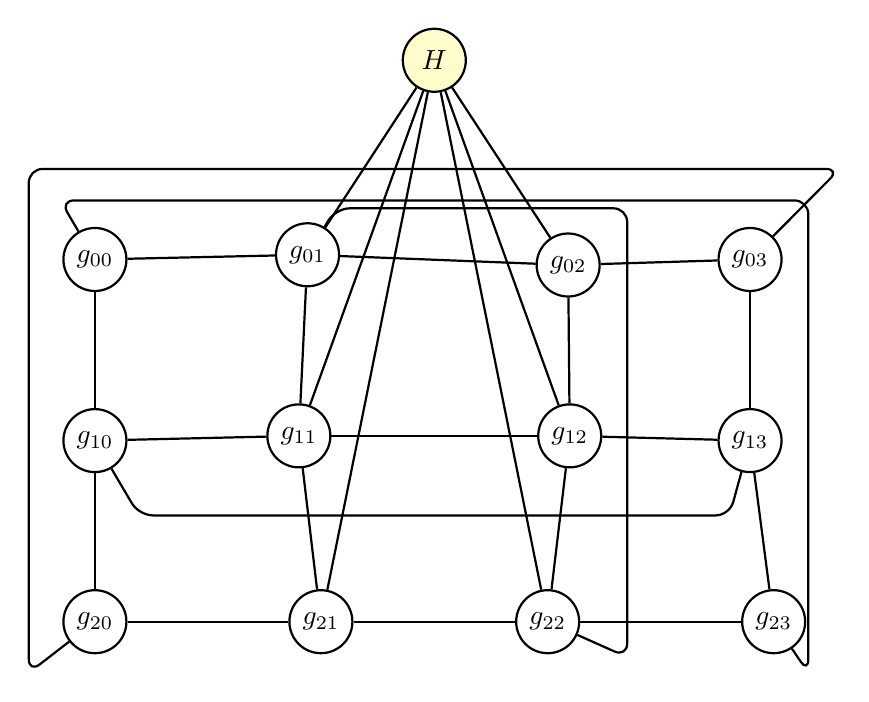
\begin{tikzpicture}[x=1cm,y=1cm]
\tikzset{
  graphnode/.style={circle,draw,thick,minimum size=8mm,inner sep=1pt,font=\sffamily},
  directed/.style={-{Stealth[length=2.4mm]},thick},
  undirected/.style={thick}
}
\node[graphnode] (n_g00) at (-0.56,0.25) {$g_{00}$};
\node[graphnode] (n_g01) at (2.14,0.31) {$g_{01}$};
\node[graphnode] (n_g02) at (5.45,0.18) {$g_{02}$};
\node[graphnode] (n_g03) at (7.76,0.25) {$g_{03}$};
\node[graphnode] (n_g10) at (-0.56,-2.05) {$g_{10}$};
\node[graphnode] (n_g11) at (2.03,-1.99) {$g_{11}$};
\node[graphnode] (n_g12) at (5.47,-1.99) {$g_{12}$};
\node[graphnode] (n_g13) at (7.76,-2.05) {$g_{13}$};
\node[graphnode] (n_g20) at (-0.56,-4.35) {$g_{20}$};
\node[graphnode] (n_g21) at (2.31,-4.35) {$g_{21}$};
\node[graphnode] (n_g22) at (5.19,-4.35) {$g_{22}$};
\node[graphnode] (n_g23) at (8.06,-4.35) {$g_{23}$};
\node[graphnode,fill=yellow!20] (n_H) at (3.75,2.78) {$H$};
\draw[undirected] (n_g00) -- (n_g01);
\draw[undirected] (n_g01) -- (n_g02);
\draw[undirected] (n_g02) -- (n_g03);
\draw[undirected] (n_g10) -- (n_g11);
\draw[undirected] (n_g11) -- (n_g12);
\draw[undirected] (n_g12) -- (n_g13);
\draw[undirected] (n_g20) -- (n_g21);
\draw[undirected] (n_g21) -- (n_g22);
\draw[undirected] (n_g22) -- (n_g23);
\draw[undirected] (n_g00) -- (n_g10);
\draw[undirected] (n_g10) -- (n_g20);
\draw[undirected] (n_g01) -- (n_g11);
\draw[undirected] (n_g11) -- (n_g21);
\draw[undirected] (n_g02) -- (n_g12);
\draw[undirected] (n_g12) -- (n_g22);
\draw[undirected] (n_g03) -- (n_g13);
\draw[undirected] (n_g13) -- (n_g23);
\draw[undirected] (n_H) -- (n_g01);
\draw[undirected] (n_H) -- (n_g02);
\draw[undirected] (n_H) -- (n_g11);
\draw[undirected] (n_H) -- (n_g12);
\draw[undirected] (n_H) -- (n_g21);
\draw[undirected] (n_H) -- (n_g22);
\draw[undirected,rounded corners=5pt] (n_g00) -- (-1.00,1.00) -- (8.50,1.00) -- (8.50,-5.00) -- (n_g23);
\draw[undirected,rounded corners=5pt] (n_g03) -- (8.90,1.40) -- (-1.40,1.40) -- (-1.40,-5.00) -- (n_g20);
\draw[undirected,rounded corners=5pt] (n_g10) -- (0.00,-3.00) -- (7.50,-3.00) -- (n_g13);
\draw[undirected,rounded corners=5pt] (n_g01) -- (2.50,0.90) -- (6.20,0.90) -- (6.20,-4.80) -- (n_g22);
\end{tikzpicture}
\end{document}
